\documentclass{proc}
\usepackage{graphicx}
\usepackage{mathtools}
\usepackage{fixltx2e}
\usepackage{algorithm}
\usepackage{algpseudocode}
\usepackage{caption}
\usepackage{url}
\usepackage{amsmath}
%\setlength{\parskip}{\baselineskip}
%\setlength{\parindent}{0pt}

\title{
The GitHub Open Source Development Process
\author{Kevin Peterson\\
Department of Information Technology\\
Clinical Informatics Support Systems\\
Mayo Clinic\\
200 1st Street\\
Rochester, MN  55905\\
\small \texttt{peterson.kevin@mayo.edu}
}
}

\begin{document}
\maketitle

\begin{abstract}
Open Source Software (OSS) projects, or software projects with publicly available source code, are realizing ever more important roles in both personal and business computing. As such, shifts in the way OSS is developed could have impacts on both the quantity and the quality of OSS projects.

The development process by which these projects are produced is generally unstructured compared to commercial software, but many projects do exhibit general development patterns. GitHub, a popular OSS code hosting website, along with Git, the site's Source Code Management (SCM) tool of choice, may have the potential to fundamentally change this process by facilitating new patterns and opportunities for developers.

By analyzing a subset of GitHub repositories, this report will show how GitHub has influenced some intrinsic aspects of traditional OSS development, such as developer hierarchies and issue close velocity. We find that many of the traditional aspects of OSS development remain, such as most project development is done by a small group of core developers. Other assumptions about project hierarchy, such as a large number of Issue Reporters compared to Committers, seems unsupported by the data.
\end{abstract}

\noindent \\\textbf{Keywords.} Git, GitHub, Open Source

\section{Introduction}
Open Source Software (OSS) has fundamentally changed how we view the Software Development Process\cite{raymond1999cathedral}. OSS projects are not only viable, but successful and thriving. 

A case study of the Apache Server project\cite{mockus2000case} shows that a dedicated community can produce software that rivals or exceeds commercial offerings. This study showed that even in the unstructured context of OSS, certain structures, hierarchies, and codes of conduct emerge. Contrast the Apache Server project to a successful project on GitHub. Although the spirit and intent may be the same, the tool set is drastically different. The intent of this work is to explore how GitHub facilitates this process, and also how it may cause it to evolve.

GitHub\footnote{https://github.com/} is a popular code hosting website that uses Git Source Code Management (SCM)\footnote{http://git-scm.com/}. GitHub... Git allows for development to take place in a more distributed manner than previously available in other SCM systems\cite{spinellis2012git}. Git also allows for a variety of work flows\cite{chacon2009pro}. These workflows may be tailored to the individual needs of a project. The Linux Kernel, for example, uses a Dictator and
Lieutenants Workflow\cite{platschekfloss}, which is hierarchical in nature. Other work flows may be more distributed, or resemble more traditional centralized SCM systems. Although work flow techniques aren't explicitly addressed in this work, it is important to note that work flow change may contribute to \textit{process change}.

To better understand quantitatively the GitHub process, three hypotheses are introduced. The goal of these hypotheses is to bridge the gap between the more qualitative research of GitHub\cite{dabbish2012social,begel2013social} and the statistical analysis of data from a random sampling of GitHub projects.

In addition, three supporting research questions are proposed. These questions will draw upon data from this work, but also reference interviews with GitHub staff to better represent how GitHub may be changing how OSS development is conducted. These qualitative observations, paired with the more qualitative data analysis, allows for a broad description of the way that GitHub is changing the Software Engineering landscape for OSS.

\subsection{Hypotheses}
The following hypotheses are presented in an effort to better understand the GitHub development process by analyzing data from actual GitHub projects. Each hypothesis will be backed by previous research in an attempt to show concrete ways in which the GitHub process may be changing the OSS development process. Where possible, results from previous research on the Apache Server[mockus2000case] is compared, as this work closely aligns with Hypothesis 2 and 3.

\noindent \textbf{Hypothesis 1: As the number of Watchers increase, the number of Repository Forks will increase.}\\
In Open Source Software, a feeling of community belonging can be intrinsically motivating to developers\cite{lakhani2003hackers}. This feeling of belonging can be expressed passively, as a \emph{watch}, or actively, as a \emph{fork} of a repository. As \emph{watches} don't necessarily signal intent to contribute, a positive direction for an OSS project is to not only increase the number of \emph{watchers}, but also the number of \emph{forks}. As both signify a general general interest in the project, it is expected that there be some correlation between the two.

\noindent \textbf{Hypothesis 2: As the number Repository Forks increase, the Issue Resolution Time will decrease.}\\
In OSS, a project \emph{fork} has at times carried negative connotations, and has even been referred to as a hazzard\cite{kogut2001open}. In the context of Git and GitHub, however, a \emph{fork} is a positive occurrence for a project, as it signifies greater project involvement. As Git allows for easy merging of \emph{forks}, code contributions in the form of defect fixes can be incorporated quickly. Because of this, it is expected that \emph{Issue Resolution Time} will decrease as the number of \emph{forks} increases.

The Apache Project noted that a rapid response to problems can be obtained because OSS is not bound to release schedules in the same way commercial software is. ``Patches'' may be released at any time, by any member of the community\cite{mockus2000case}. ``Patches'' in the context of GitHub could be equated to Pull Requests.

This is, ultimately, a proof of ``Linus Law"\cite{raymond1999cathedral} in the context of GitHub. In other words, the more exposure the code gets (in terms of forks), the easier bugs will be to find and fix.

\noindent \textbf{Hypothesis 3: There will be more Issue Reporters than Committers by an order of magnitude}\\
Research into the Apache Server project observed that there were far more \emph{Issue Reporters} than there were code \emph{Committers}\cite{mockus2000case}. The Apache Server project is an excellent case study in this type of Developer Hierarchy. Apache is built around a small set of {\it Core Developers}, followed by {\it Defect Repairers} and {\it Defect Reporters}. Each level of this hierarchy brings with it an order of magnitude increase in number of participants. The 10-15 {\it Core Developers} contribute around 80\% of the new functionality, while the rest of the 400 code contributors focus primarily on bug fixes. The {\it Defect Reporters} were by far the largest group, with over 3000 individuals submitting bug reports.

Because issue reporting is of low risk to the code base, but has potentially high value, it is a perfect way for large numbers of people to contribute. It is expected that the findings of the Apache Server project research will hold true for GitHub projects as well.

\subsection{Research Questions}
To expand the analysis scope slightly, three qualitative research questions are posed. These, although backed by analyzed data where possible, are intended to show broader patterns, ideas, and motivations around the use of GitHub. Where possible, interviews\cite{begel2013social} where conducted to explore high level concepts and motivations.

\noindent \textbf{Research Question 1: Are GitHub projects primarily focused around a small set of core Committers?}\\
A smal core of developers, however, seems to be a historical fact of OSS development\cite{mockus2000case,mockus2002two,krishnamurthy2002cave}. At the extreme of this, a study of projects on the software hosting site Sourceforge\footnote{http://sourceforge.net} found that a large percentage of OSS development is done by lone developers. Is a small core of developers intrinsic to OSS development, or have the social aspects of GitHub and the distributed nature of Git changes this?

\noindent \textbf{Research Question 2: How is GitHub changing the OSS process?}\\
The social aspects of GitHub are an important part of the experience\cite{dabbish2012social}. User interactions and social pressures can drive OSS development in interesting ways. Social aspects of OSS development have existed before GitHub, with mailing lists\cite{mockus2000case}, gift giving mechanisms\cite{bergquist2008power}, and other code hosting sites. What is GitHub doing to facilitate change on OSS development, and how does it see OSS development changing moving forward?

\noindent \textbf{Research Question 3: Can GitHub be used for more that code artifacts?}\\
The Object Management Group\textregistered\footnote{http://www.omg.org} computer industry consortium focused on technology standards. Potential standard submission teams must go through a vetting process\cite{kobryn1999uml} which allows industry representatives to provide feedback on the standard. Gathering and recording this feedback is a challenge, but GitHub's issue tracking system may be able to streamline the process.

\section{Methods}
\subsection{Collection and Storage}
Data collection was done using the GitHub REST API\footnote{http://developer.github.com/v3/}. A random selection of 1000 repositories was selected using Algorithm \ref{algo:data_collection_algo}.

\begin{algorithm}[H]
\captionof{algorithm}{Data Collection Algorithm}\label{algo:data_collection_algo}
\begin{algorithmic}[1]
\While{$i < 1000$} 
\State $i \gets i + 1$
\State $word \gets random(word\_list)$
\State $repos \gets git\_search(word)$
\State $j \gets $%\Call{random}{0... \Call{size}{repos}}$
\State $repo \gets repos_j$
\State \Call{store}{repo}
\EndWhile
\end{algorithmic}
\end{algorithm}

The \textsc{store} function accepts as an input a given random repository. The purpose of this function is to persist the given repository to a database for further analysis. Results were stored in a MySQL relational database management system. The database schema to store the data is described in Figure \ref{fig:er_diagram}.

\begin{figure}
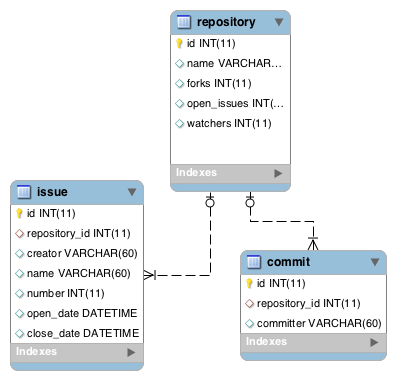
\includegraphics[height=3in,width=3in]{images/er.png}
\caption{GitHub Date Entity Relationship diagram}
\label{fig:er_diagram}
\end{figure}

Data was collected and analyzed using a Python\footnote{http://python.org/} script. Because the GitHub REST API constrains the number of API calls per hour made by a client, logic was included to pause execution when the allotment was exhausted.

Matplotlib\cite{Hunter2007}, a 2D graphics package for Python, was used to render graphs and charts. NumPY and SciPY\cite{scipy} were used for data analysis calculations, such as correlation coefficients.

All source code and materials used in data collection and analysis are hosted at GitHub (naturally!), and may be accessed by the following URL: \url{https://github.com/kevinpeterson/github-process-research}

\subsection{Analysis}
In this context, a \textit{Repository} is defined as a Set of \textit{Attributes}. An \textit{Attribute} is a metric of interest. See Section \ref{sec:attributes} for further information on individual \textit{Attributes}. These metrics of interest are used as an Indexing Set $A^\prime$, and have labels as follows:

\[A^\prime = \{i, c, i^\prime, i^{\prime\prime}, \Delta, \alpha, \beta\}\]

Where $i$ = {\textit{Issues}, $c$ = {\textit{Commits}, $i^\prime$ = {\textit{Closed Issues}, $i^{\prime\prime}$ = {\textit{Open Issues}, $\Delta$ = {\textit{Issue Close Time}, $\alpha$ = {\textit{Issue Creators}, and $\beta$ = {\textit{Committers}.

All analyzed \textit{Respositories} can be thought of as the Indexed Family of \textit{Attribute} Sets $A$, or a Set of Sets of \textit{Attributes}. Let the Set of these Sets of \textit{Attribute} Sets be called $S$, or the \textit{Repository Sample}. We can label the \textit{Attribute} Sets by arbitrary integers 0 through $|S|$, or:
\[ \{A_i\}_{i \in \{0,1,2 ... |S|\} }\]

In this way, we can reference a Set of \textit{Attributes} (or, an individual \textit{Repository}), by $A_i$. 

Going further, we can also denote an individual \textit{Attribute} of a given \textit{Repository} by:
\[ \{A_{(i,r)}\}_{(i,r) \in A^\prime \times \{0,1,2 ... |S|\} } \]
or, $A_{i,r}$. For example, $A_{\Delta,10}$ would denote the value of the \textit{Issue Close Time} ($\Delta$) of Repository \textit{10}.

Each individual Attribute processed by some aggregate function $f$, or $f(  A_{i,r} )$. For this analysis, the aggregate functions are: \textsc{mean}, \textsc{min}, \textsc{max}, \textsc{stddev}. This analysis is applied to all $n$ repositories for which data was collected. Results were then averaged over all repositories. Each attribute is analyzed independently, so given:
\[ g(j) = \frac{\sum\limits_{r = 0}^{|S|} f(  A_{r,j}  ) }{|S|} \]
each individual attribute is processed via $g(j)$ and will result in the average of the given aggregate function.

\subsubsection{Attributes}
\label{sec:attributes}
The individual \textit{Attribute} names, or the elements of $A^\prime$, are described below. For detailed summary statistics of these \textit{Attributes}, see Figure  \ref{table:summary_stats}.\\\\
\noindent \textbf{\textit{Issues:}}
The number of issues posted to a repository's issue tracker\footnote{https://github.com/blog/411-github-issue-tracker}.

\noindent \textbf{\textit{Commits:}}
The number of individual source code commits to a repository. It is important to note that a textit{commit} is a single transaction that changes the code contents of a repository. Actual commit ``size'' (lines of code modified, for example), is not taken into account.

\noindent \textbf{\textit{Closed Issues:}}
The number of issues in a repository in a state of \textsc{closed} at the time of processing.

\noindent \textbf{\textit{Open Issues:}}
The number of issues in a repository in a state of \textsc{open} at the time of processing.

\noindent \textbf{\textit{Issue Close Time:}}
The average time taken to close a given issue in a repository. Non-\textsc{closed} issues were not counted.\\

The average is calculated using the following method. Let $d(x)$ be a function that converts seconds to a Date, and let $s(x)$ be a function that converts a Date to seconds. Let $I$ equal the Set of \textit{Issues} in a given repository, with elements comprised of tuples $(\tau, \tau^\prime)$, where $\tau$ is \textit{Issue Open Time} and $\tau^\prime$ is \textit{Issue Close Time}. We calculate \textit{Issue Close Time} by: 

\[ \Delta = d\left( \frac{\sum_{i \in I} s( p_{(1)}i ) - s( p_{(2)}i )  } {n} \right) \]

Where for each issue $i$ in $I$, the \textit{Issue Open Date} $s( p_{(1)}i)$ is subtracted from the \textit{Issue Close Date} $s( p_{(2)}i)$, and $p_{(1)}i$ and $p_{(2)}i$ denote the elements of the tuple, or \textit{Issue Open Date} and \textit{Issue Close Date}, respectively. The result of this is averaged and converted into a Date via $d(x)$, resulting in the average issue close time interval $\Delta$.

\noindent \textbf{\textit{Issue Creators:}}
The number of distinct users that have opened at least one \textit{Issue}.

\noindent \textbf{\textit{Committers:}}
The number of distinct users that have summited at least one \textit{Commit}.

\section{Results}

\subsection{Summary Statistics}
\begin{table}[!ht]
\begin{center}
\begin{tabular}{rrrrrrr}
\hline
Variable & Mean & Min & Max & Std. Dev. \\
\hline
Issues  &  30.93  &  1  &  860  &  83.18  \\
Commits  &  249.3  &  1  &  45379  &  1700.01  \\
Closed Issues  &  26.6  &  1  &  837  &  77.56  \\
Open Issues  &  11.37  &  1  &  316  &  31.63  \\
Issue Close Time  &  26.48  &  0  &  503  &  56.54  \\
Issue Creators  &  10.61  &  1  &  128  &  22.29  \\
Committers  &  4.8  &  1  &  405  &  16.39  \\

\hline
\end{tabular}
N = 1000 Repositories
\caption{GitHub Summary Statistics}
\label{table:summary_stats}
\end{center}
\end{table}

Table \ref{table:summary_stats} describes summary statistics of the repository variables above. The most evident feature of the result is the large variance. In fact, for the set of tested variables $A$, each variable $A_j$ is observed to have a larger standard deviation than the variable mean.
\begin{equation}
\forall j \in A \colon \overline{j} < \sigma_{j}
\label{eq:variance}
\end{equation}
All measured variables demonstrated this characteristic.

The sample ($N = 1000$) GitHub repositories were analyzed, out of a total of 5.7 million\cite{githubPress}.

\subsection{Hypotheses}
\textbf{Hypothesis 1: As the number of Watchers increase, the number of Repository Forks will increase.}\\
A correlation coefficient of 0.938794181553 was observed between the number of Watchers and Forks of a repository. This suggests that a correlation between Watchers and Forks exists.

\begin{figure}
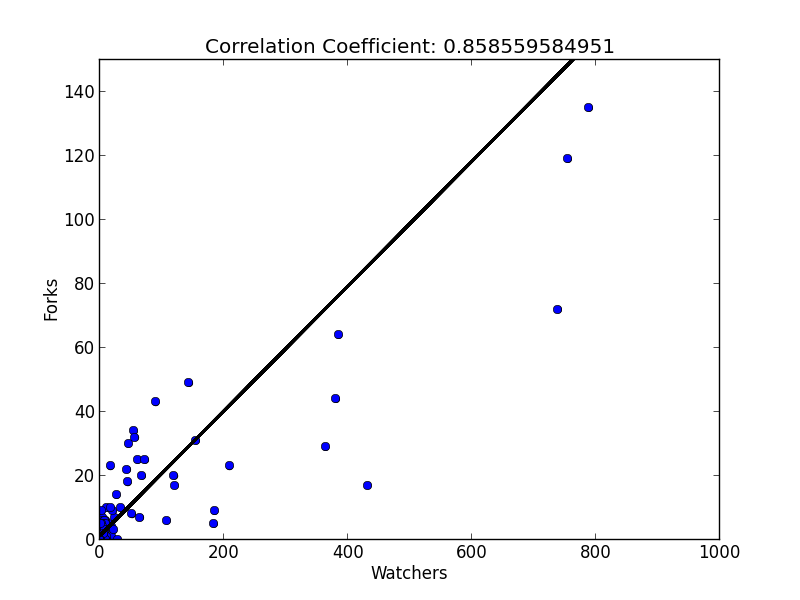
\includegraphics[height=3in,width=3in]{images/watcher_forks_scatterplot.png}
\caption{Repostitory watchers and forks}
\end{figure}

The data reinforces the hypothesis, as does other research in the area. Even though there are arguments that the number of Forks is the true measure of project success\cite{baudry2012towards}, the data suggests that the two measures are related. Also, \textit{Dabbish et al.} have noted that the number of Watches can be a key for others to gauge interest in a project, and thus determine if they should participate \cite{dabbish2013leveraging}. If the number of Watchers of a repository serves as a social cue for participation, even ``passive'' involvement with a project (Watching) could influence the ``active'' participation (Forking). This could possibly contribute to the correlation of the two variables.\\

\textbf{Hypothesis 2: As the number Repository Forks increase, the Issue Resolution Time will decrease.}\\
No significant correlation was found between the number of repository forks and issue resolution time. It is important to note, however, that issue resolution time is not necessarily related to software product quality in the context of GitHub. We can assert that for serveral reasons. \textit{First}, GitHub issues are not necessarily product defects. Issues may be feature requests. TODOs, or general support questions. \textit{second}, GitHub projects may have primary issue tracking services elsewhere, while using the GitHub issues as secondary services or not at all. \textit{Third}, Pham \textit{et al.} explore an emerging ``testing culture'' in GitHub -- something which could have sizable impacts on software quality but wouldn't necessarily be reflected in this metric \cite{phamcreating}.

\begin{figure}
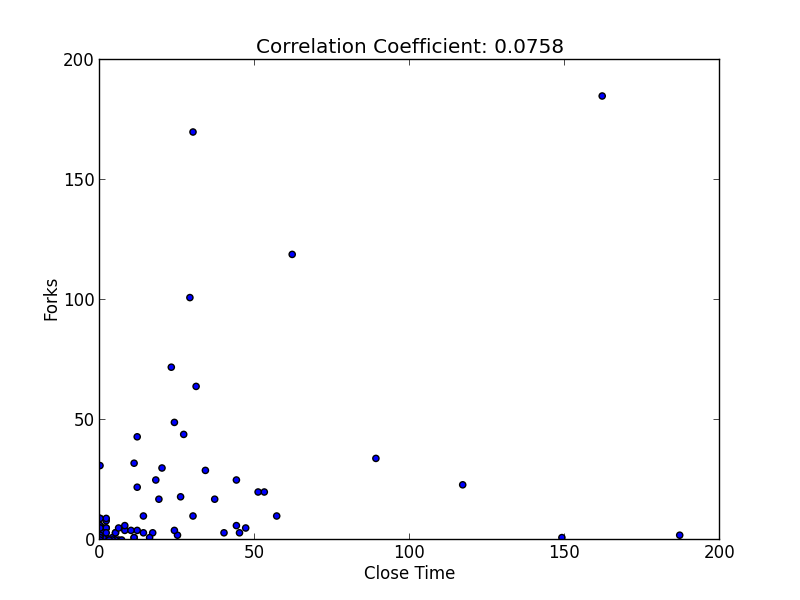
\includegraphics[height=3in,width=3in]{images/issue_close_time_forks_scatterplot.png}
\caption{Repostitory issue close time and number of forks}
\label{fig:issue_close_time_forks_scatterplot}
\end{figure}

It is possible that other factors, such as issue prioritization, may have a greater impact on issue resolution time. Research does support a relationship\cite{mockus2002two} between the stated priority and fix interval. As the GitHub issue tracker can only support prioritization by free-text \textit{tags} placed on issues, it is not feasable to programmattically gather issue priority metrics.\\

\textbf{Hypothesis 3: There will be more Issue Reporters than Committers by an order of magnitude.}\\
Data does not support an exponentially increasing number of distinct Issue Reporters as compared to distinct Committers. 
As shown in Figure\ref{fig:issue_reporters_committers_scatterplot}, the slope of the relationship between the two variables is less than one. This does not seem to completely align with findings in the Apache Server project\cite{mockus2000case}. 

\begin{figure}
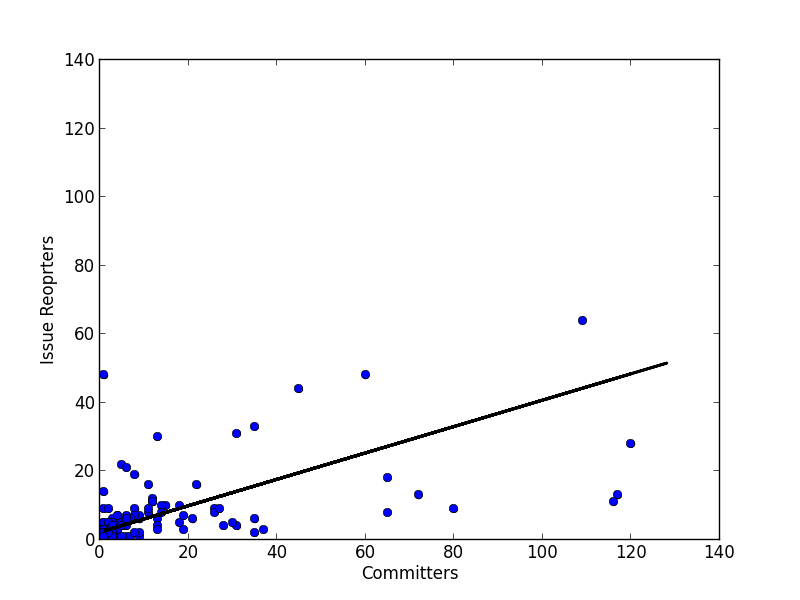
\includegraphics[height=3in,width=3in]{images/issue_reporters_committers_scatterplot.png}
\caption{Repostitory issue reporters and committers}
\label{fig:issue_reporters_committers_scatterplot}
\end{figure}

Figure\ref{fig:issue_reporters_committers_scatterplot}, does however suggest, however, that that the two variables may be related. The hypothesis implies that there will be a correlation between the two variables -- which is demonstrated by a reasonably strong correlation cofficient of 0.8299. More investigation would be necessary to further examine this finding.\\

\subsection{Research Questions}
\textbf{Research Question 1: Are GitHub projects primarily focused around a small set of core Committers?}\\
The data in figure \ref{fig:committers_percentage_pie_chart} represents commit percentage breakdown. The inner percentages represent the percentage of committers in a project that that have committed the outer percentage amount of commits to that project, or:

\begin{equation}
P = \left\{ \frac{ C_u } { |C| } \times 100 \Big| u \in U \right\}
\label{eq:commit_percentage}
\end{equation}

Where $U$ is the Set of \textit{Committers} to a given \textit{Repository} and $C$ is the MultiSet of \textit{Commits} by an individual \textit{Committers} to a given \textit{Repository}, or:
 \[ \{ C_u \}_{u \in U} \]

\begin{figure}
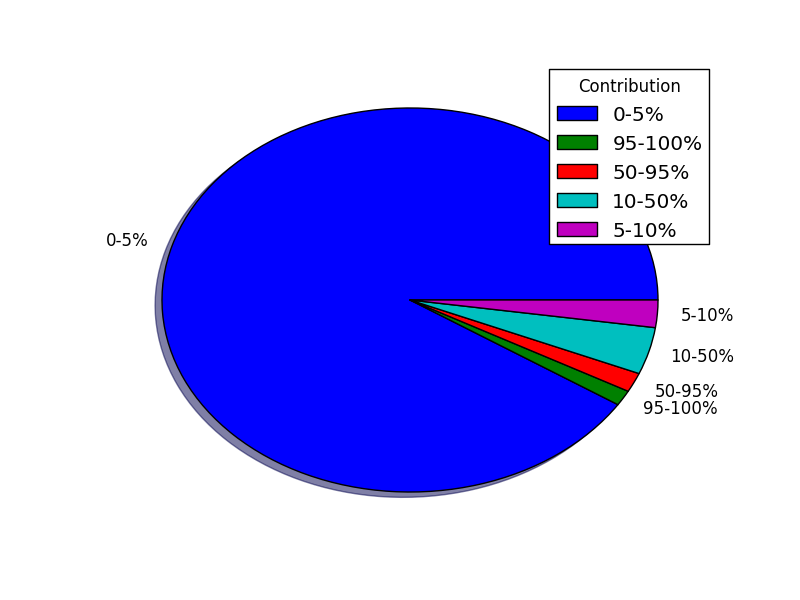
\includegraphics[height=3in,width=3in]{images/committers_percentage_pie_chart.png}
\caption{Individual committer commit percentage per repository}
\label{fig:committers_percentage_pie_chart}
\end{figure}

To find the percentages Set $P$ of equation\ref{eq:commit_percentage}, the commits by each user $C_u$ are divided by the total number of commits $|C|$, yielding the set of contribution percentages $P$ for the repository. Elements of $P$ are then assigned to ranges $0-5\%$, $5-10\%$, $10-50\%$, $50-95\%$, and $95-100\%$ (with shared values inclusive to the larger range). The distribution of this range assignments is plotted on Figure \ref{fig:committers_percentage_pie_chart}.

There does appear to be evidence of a small set of core developers, denoted by the relatively high percentage of developers that have authored $95-100\%$ of the commits of a given repository. Most notably, however, is that the data shows that by a large percentage of developers committed small amounts ($0-5\%$ of the total repository commits). This means that a small core are not entirely monopolizing the commits, but rather opportunity exists for users to contribute, even if in small ways.

\begin{figure}
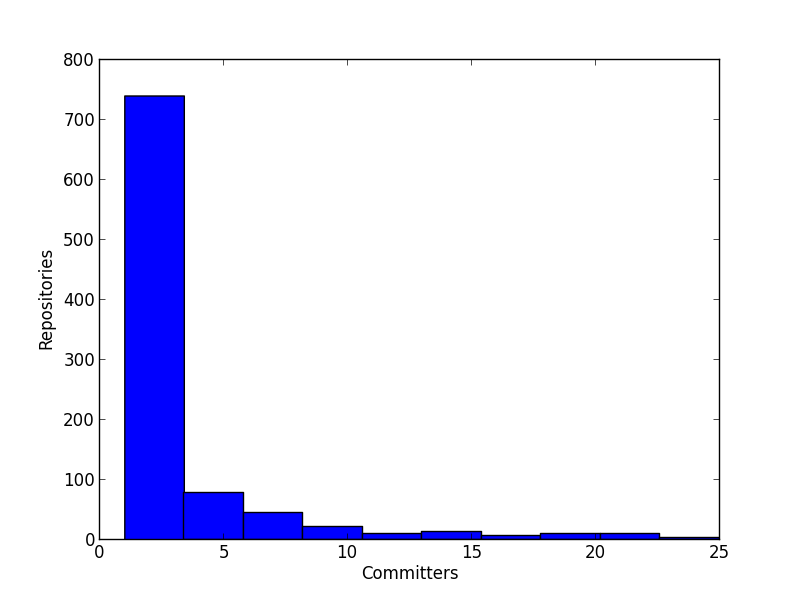
\includegraphics[height=3in,width=3in]{images/committers_histogram.png}
\caption{Count of individual committers per repository}
\label{fig:committers_histogram}
\end{figure}

When looking strictly at the number of committers to a repository, however, the notion of a small set of core Committers is strongly supported, as the vast majority of repositories have fewer than 10 committers (figure \ref{fig:committers_histogram}).\\

\textbf{Research Question 2: How is GitHub changing the OSS process?}\\
Thung \textit{et al.} show that the social coding aspects of GitHub -- specifically the developer-to-developer connectivity -- enable high collaboration rates.\cite{thung2013network} In fact, the developer connectivity was shown to be higher than SourceForge and even Facebook. In a recent interview with GitHub staff, the social aspects of GitHub are referred to as ``unique and powerful\cite{begel2013social},'' which seems to suggest that this is a strong underlying product goal for.

Ye also observed\cite{ye2003toward} that the contribution environment, or ``society,'' is important in providing a framework for develper trust building:
\begin{quote}
Only in a society where technical supremacy is highly appreciated can developers acquire good reputations among their peers by displaying their skills through free distribution, and often wider acceptance, of their systems.The good reputation attracts attention, trust, and cooperation from others and lays the foundation for advancing the original developers agenda and the establishment and development of OSS communities. 
\end{quote}

To further analyze this research question, and to explore further the GitHub ``society'' and its impact on OSS development, an interview with GitHub staff was conducted.\\\\
\textit{Interview Q1: How is GitHub changing the way OSS is being developed?}\\

\textit{Interview Q2: Many new Software Developers are will be starting their education/training already having experience with GitHub. How will Software Engineering as a discipline (and how it is taught) change to accommodate the ideas popularized by GitHub?}\\

\textit{Interview Q3: There are many non-code artifacts being hosted on GitHub, for example, Object Management Group Specifications, Laws and Statutes, books... etc. Do you see GitHub participation expanding in the non-code areas?}\\

\textbf{Research Question 3: Can GitHub be used for more that code artifacts?}\\
The OMG\textregistered standardization process is a process by which products strive to produce an interoperability statndard by way of an industry standards consortium.\cite{omgTechProcess}
The standardization process itself aims to, at its conclusion, produce a set of model artificats containing sufficient detail such that when interpreted and implemented, produce interoperable software.
At a conceptual level, this can be thought of as a software requirements engineering process as much as a standardization process. If so,  of the five main tasks of requirements engineering, Elicitation, Analysis and Negotiation, Documentation, Validation, and Management,\cite{sommerville1998requirements} we can show that GitHub is an appropriate forum for many of them.

As a case study, the CTS2 OMG\textregistered Specification\cite{cts2} used a GitHub issue tracker\footnote{https://github.com/cts2/cts2-specification/issues} to track specification changes. Elicitation, Analysis and Negotiation were natural fits for the issue tracker. This was chosen in part because the barrier to participation was very small (only a GitHub account was needed), and issues tracker itself allowed for dialogs in the form of comments. Because customer involvement is critical to these activities\cite{paetsch2003requirements}, ease of contribution was a main concern. OMG has a predescribed format for requirements Documentation, but using the GitHub issue API\footnote{http://developer.github.com/v3/issues/}, much of this documentation can be automated.
Validation and Management are areas of requirements engineering that GitHub has interesting solutions for. First, in order to track (or validate) changes to the specification, when the actual specification is modified, the commit that modified it can be traced to a named issue by simply putting the issue number in the commit log. This level of traceability is powerful, as it allows every change to the specification artifacts to be tracked consistently to an open issue. As the normal OMG process proceeds, requirements can be managed through ``tagging'' the issues. By allowing issues to be grouped by arbitrary tags, users are more free to adapt their own workflow. For instance, when community voting on issues needed to be done for CTS2, a simple ``ready for vote'' tag signified to the voting board exactly what was under consideration

As mentioned, the CTS2 specification made heavy use of the GitHub issue tracker, as well as another OMG specification, ServD\footnote{https://github.com/servd/servd-specification}. For open source specifications, or requirements engineering activities, GitHub has shown to be a viable platform. 

\section{Conclusion}

\section{Acknowledgments}

\bibliographystyle{plain}
\bibliography{bibliography}

\end{document}